\documentclass{beamer}

\mode<presentation> {

\usetheme{default}
\usecolortheme{default}

%\setbeamertemplate{footline} % To remove the footer line in all slides uncomment this line
%\setbeamertemplate{footline}[page number] % To replace the footer line in all slides with a simple slide count uncomment this line
%\setbeamertemplate{navigation symbols}{} % To remove the navigation symbols from the bottom of all slides uncomment this line
}

\usepackage{graphicx} % Allows including images
\usepackage{booktabs} % Allows the use of \toprule, \midrule and \bottomrule in tables
\usepackage{soul}
\makeatletter
\newcommand\SoulColor{%
  \let\set@color\beamerorig@set@color
  \let\reset@color\beamerorig@reset@color}

\setbeamertemplate{caption}{\insertcaption} 
\setbeamertemplate{caption label separator}{}
\setbeamerfont{frametitle}{size=\Large}

\newenvironment{graytext}{\color{gray}}{\ignorespacesafterend}

%----------------------------------------------------------------------------------------
%	TITLE PAGE
%----------------------------------------------------------------------------------------

\title[Traveling for mates]{Are sex differences in mobility all about mating?} % The short title appears at the bottom of every slide, the full title is only on the title page

\author{Layne J. Vashro} % Your name
\institute[Utah] % Your institution as it will appear on the bottom of every slide, may be shorthand to save space
{
University of Utah \\ % Your institution for the title page
\medskip
\textit{Layne.Vashro@anthro.utah.edu} % Your email address
}
\date{\today} % Date, can be changed to a custom date

\begin{document}

\begin{frame}
\titlepage % Print the title page as the first slide
\end{frame}

%------------------------------------------------

%\begin{frame}<beamer>{Table of Contents}
%\tableofcontents[hidesubsections]
%\end{frame}

%------------------------------------------------
%------------------------------------------------

\section{Introduction}

%------------------------------------------------
%------------------------------------------------

\begin{frame}
\frametitle{Sexual dimorphism}

\begin{columns}
\begin{column}{.5\textwidth}

Spatial ability, orientation, navigation, anxiety... \\
\vspace{0.75cm}
Range size? \\

\end{column}

\begin{column}{.5\textwidth}
\includegraphics[width= 1\textwidth]{hum_di}
\end{column}

\end{columns}

\end{frame}

%------------------------------------------------

\begin{frame}
\frametitle{Looking for mates? }

\begin{columns}
\begin{column}{.5\textwidth}

Hunting, warfare, energy and risk \\
\vspace{0.75cm}
Mating system and ranging \\
\vspace{0.75cm}
Humans? \\

\end{column}

\begin{column}{.5\textwidth}
\includegraphics[width= 1\textwidth]{dimorph}
\end{column}

\end{columns}

\end{frame}

%------------------------------------------------
%------------------------------------------------

\section{Methods}

%------------------------------------------------
%------------------------------------------------

\begin{frame}

\frametitle{Twe}

\begin{columns}
\begin{column}{.5\textwidth}
\includegraphics[width= .9\textwidth]{bigmap}
\end{column}

\begin{column}{.5\textwidth}
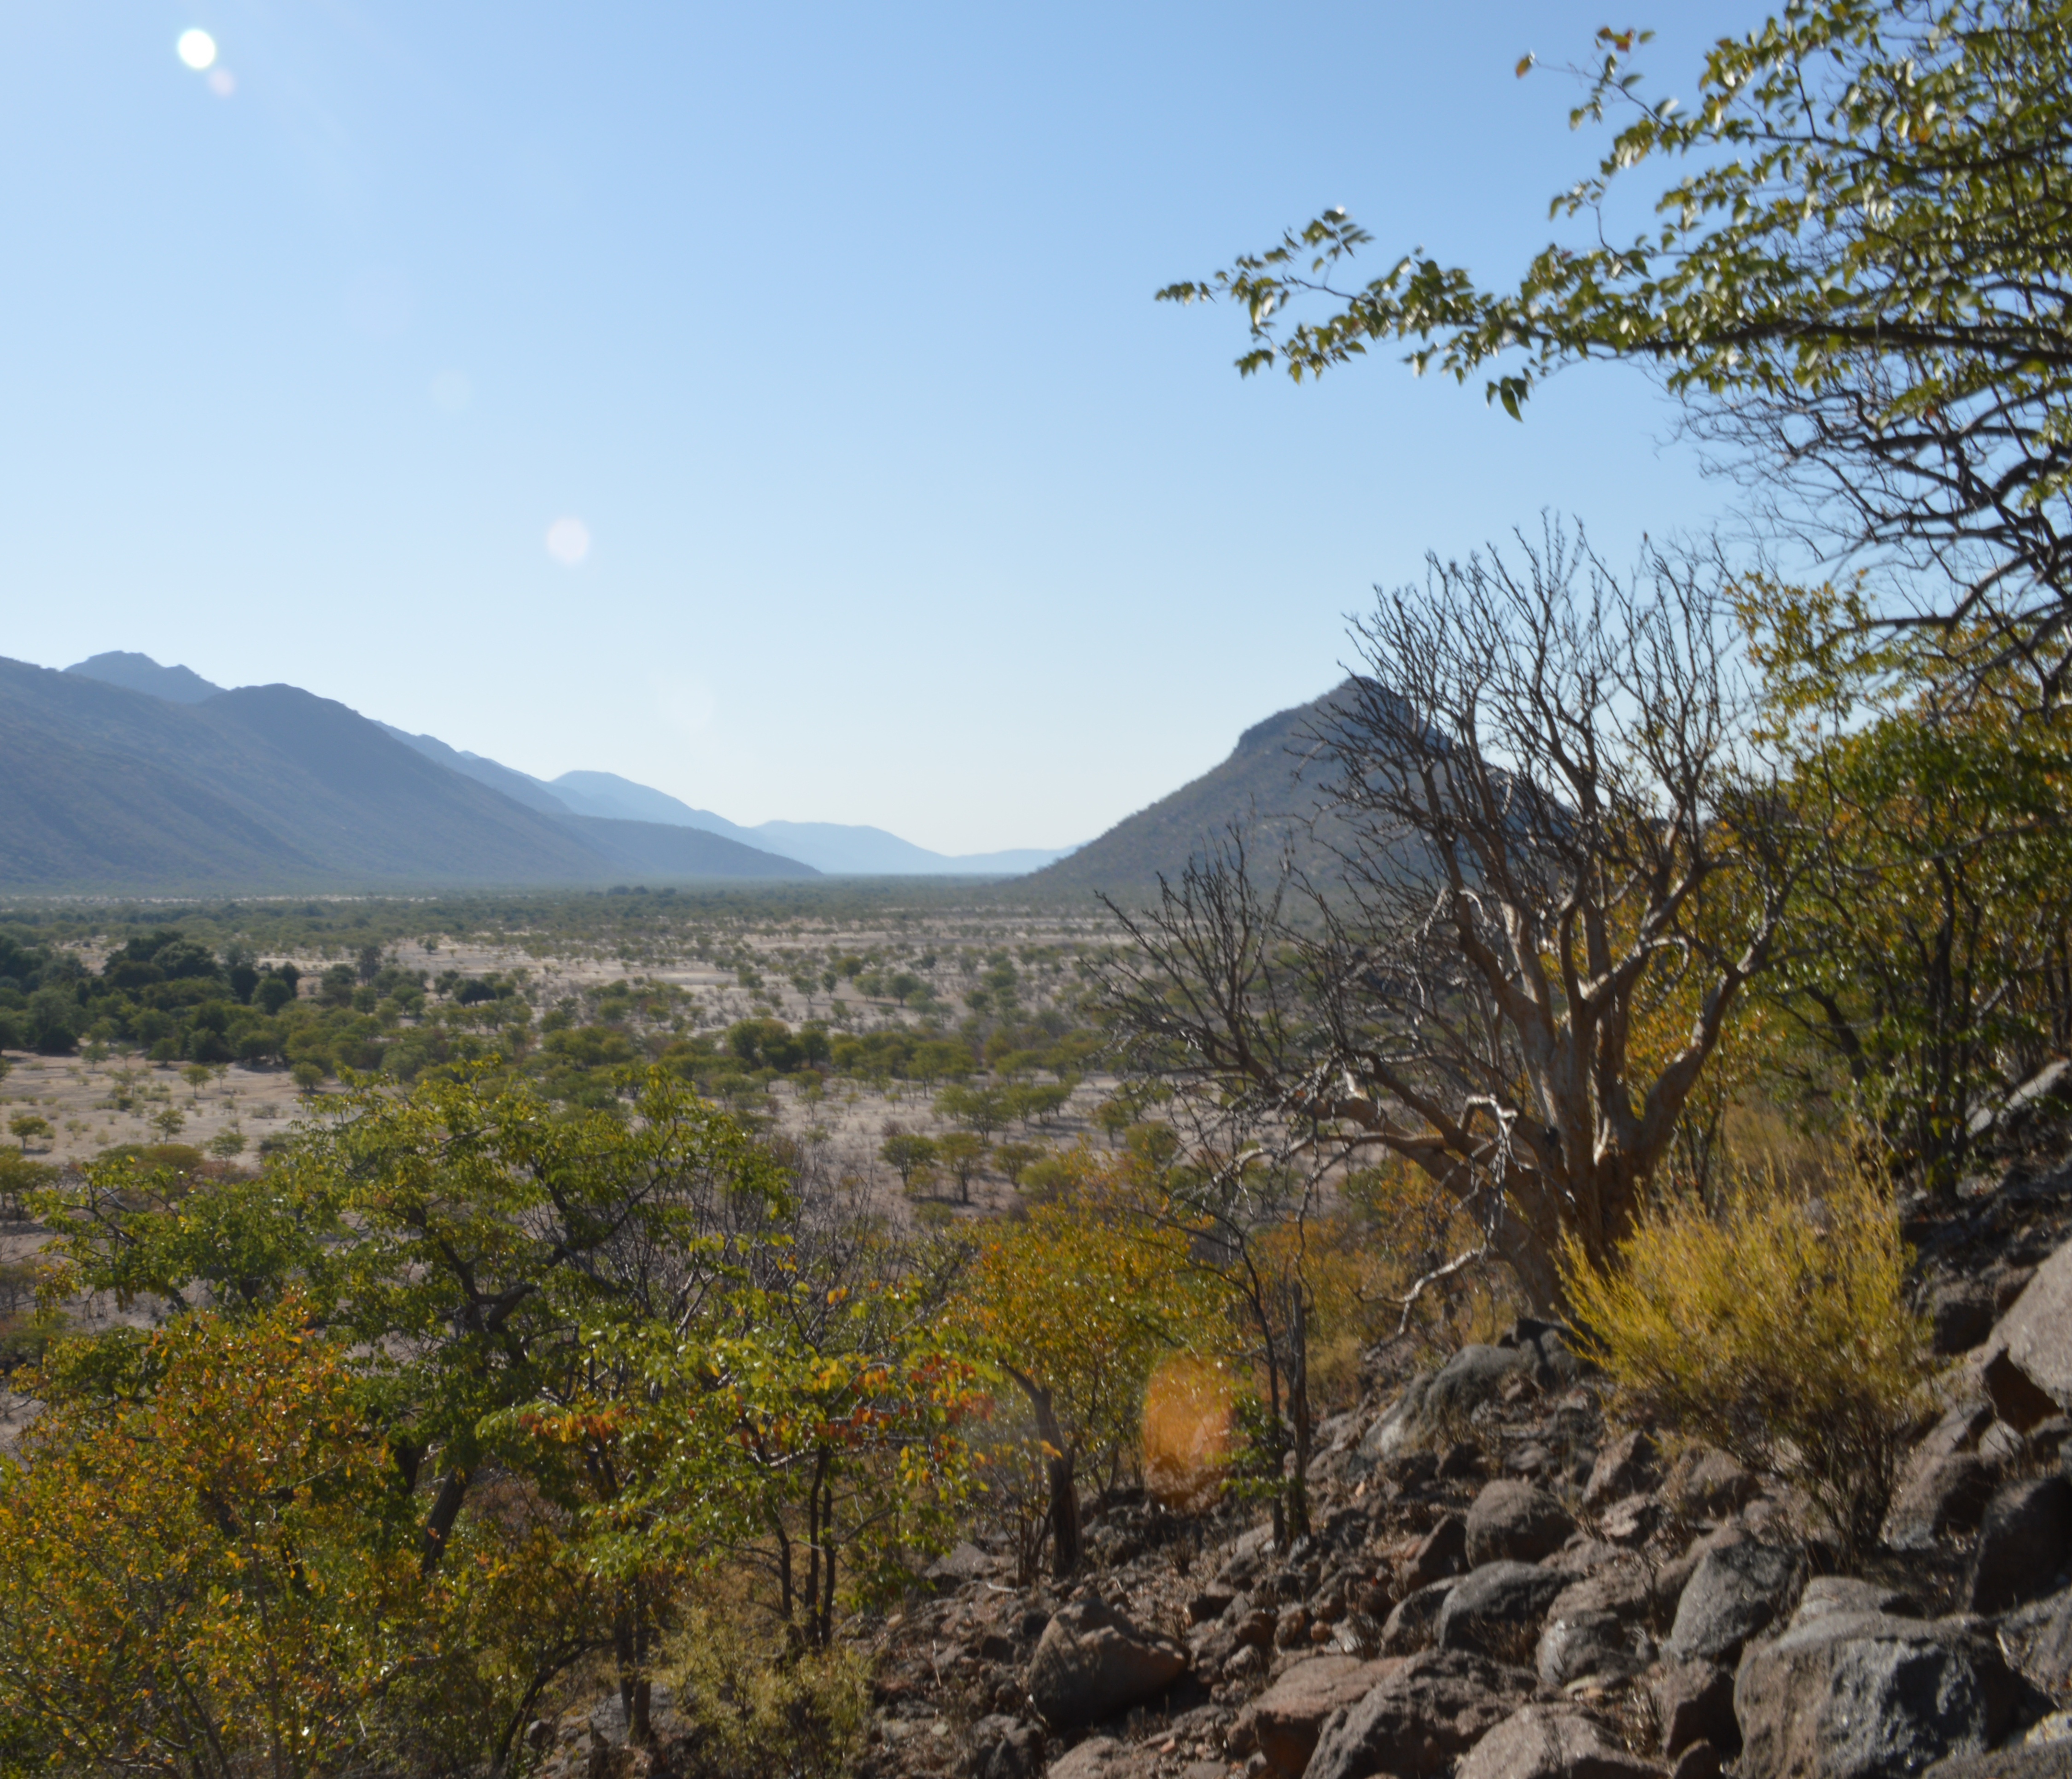
\includegraphics[width= .8\textwidth]{zebras}
\vspace{0.15cm}
\includegraphics[width= .8\textwidth]{twe_couple}
\end{column}

\end{columns}

\end{frame}

%------------------------------------------------

\begin{frame}
\frametitle{Mobility Measures}

\begin{columns}
\begin{column}{.5\textwidth}
Daily: GPS tracking \\
-- MCP km$^{2}$ \\
\vspace{0.75cm}

Annual: Travel interviews \\
-- Unique visits \\
-- How many times? \\
-- w/to whom? Why? Lover? \\
\vspace{0.75cm}

Lifetime: Regional checklist \\
-- Once? Few? Many? (Ordinal)
\end{column}

\begin{column}{.5\textwidth}
\includegraphics[width= 1\textwidth]{MCP}
\end{column}

\end{columns}

\end{frame}

%------------------------------------------------

\begin{frame}

\frametitle{Hypotheses}

H1: Twe men occupy larger ranges than women \\
\vspace{0.75cm}
H2: The sex difference in travel is explained by mate searching \\
\vspace{0.75cm}
H3: Range size predicts RS among men, but not women \\

\end{frame}

%------------------------------------------------
%------------------------------------------------

\section{Results}

%------------------------------------------------
%------------------------------------------------

\begin{frame}
\frametitle{Results: [H1] Do men travel more than women?}

\begin{columns}
\begin{column}{.5\textwidth}
\includegraphics[width= .8\textwidth]{dispersal}
\end{column}

\begin{column}{.5\textwidth}
\includegraphics[width= 1\textwidth]{tjokwalk}
\end{column}

\end{columns}

\end{frame}

%------------------------------------------------

\begin{frame}
\frametitle{H1}
\begin{table}
\begin{tabular}{lrrrrrrr}
\hline\noalign{\smallskip}
Measure & $M_{m}$ & $SD_{m}$ && $M_{f}$ & $SD_{f}$ && p \\
\noalign{\smallskip}\hline\noalign{\smallskip}
\SoulColor\hl{Daily (km$^{2}$ )} & 49.6 & 30.3 && 22.6 & 10.9 && .001 \\
Annual (locations) &&&&&&&\\
Lifetime (0:3) &&&&&&& \\
\noalign{\smallskip}\hline
\end{tabular}\par
\end{table}		  

\end{frame}

%------------------------------------------------

\begin{frame}
\frametitle{H1: Daily range}

\begin{columns}
\begin{column}{.5\textwidth}
\includegraphics[width= 1\textwidth]{mobrng_sex}
\end{column}

\begin{column}{.5\textwidth}
\includegraphics[width= 1.1\textwidth]{dailyage}
\end{column}

\end{columns}

\end{frame}

%------------------------------------------------

\begin{frame}
\frametitle{H1}
\begin{table}
\begin{tabular}{lrrrrrrr}
\hline\noalign{\smallskip}
Measure & $M_{m}$ & $SD_{m}$ && $M_{f}$ & $SD_{f}$ && p \\
\noalign{\smallskip}\hline\noalign{\smallskip}
Daily (km$^{2}$ ) & 49.6 & 30.3 && 22.6 & 10.9 && .001 \\
\SoulColor\hl{Annual (locations)} & 4.4 & 4.0 && 2.3& 1.5 && .003 \\
Lifetime (0:3) &&&&&&& \\
\noalign{\smallskip}\hline
\end{tabular}\par
\end{table}		  

\end{frame}

%------------------------------------------------

\begin{frame}
\frametitle{H1: Annual travel}

\begin{columns}
\begin{column}{.5\textwidth}
\includegraphics[width= 1\textwidth]{mobtot_sex}
\end{column}

\begin{column}{.5\textwidth}
\includegraphics[width= 1.1\textwidth]{annualage}
\end{column}

\end{columns}

\end{frame}

%------------------------------------------------

\begin{frame}
\frametitle{H1}
\begin{table}
\begin{tabular}{lrrrrrrr}
\hline\noalign{\smallskip}
Measure & $M_{m}$ & $SD_{m}$ && $M_{f}$ & $SD_{f}$ && p \\
\noalign{\smallskip}\hline\noalign{\smallskip}
Daily (km$^{2}$ ) & 49.6 & 30.3 && 22.6 & 10.9 && .001 \\
Annual (locations) & 4.4 & 4.0 && 2.3 & 1.5 && .003 \\
\SoulColor\hl{Lifetime (0:3)} & 1.5 & 0.6 && 1.0 & 0.5 && .000 \\
\noalign{\smallskip}\hline
\end{tabular}\par
\end{table}		  

\end{frame}


%------------------------------------------------


\begin{frame}
\frametitle{H1: Lifetime range}

\begin{columns}
\begin{column}{.5\textwidth}
\includegraphics[width= 1\textwidth]{mobltm_sex}
\end{column}

\begin{column}{.5\textwidth}
\includegraphics[width= 1.1\textwidth]{ltage}
\end{column}

\end{columns}

\end{frame}

%------------------------------------------------

\begin{frame}
\frametitle{H2: Do men travel to visit mates?}

\begin{columns}
\begin{column}{.6\textwidth}
Travel has many functions \\
\vspace{0.75cm} 
Do traveling men find more mates? \\
\vspace{0.75cm} 
Does mate searching explain sex difference? \\
\vspace{0.75cm} 

\end{column}

\begin{column}{.4\textwidth}
\includegraphics[width= 1\textwidth]{travelmate}
\end{column}

\end{columns}

\end{frame}


%------------------------------------------------

\begin{frame}
\frametitle{H2: Do men travel to visit mates?}

\begin{columns}
\begin{column}{.6\textwidth}
24\% locations visited by men had lovers. \\
\vspace{0.75cm} 
13.5\% of visits explicitly for mating \\
\vspace{0.75cm} 
Only loveless trips sex-diff drops .5 \\
\vspace{0.75cm} 
Lovers and frequented locations \\
%``Many'' 54.5\% if lover, 20\% if not
%5:50, mating explains 34\%:40\% of trip

\end{column}


\begin{column}{.4\textwidth}
\includegraphics[width=1\linewidth]{mobmat_sex}
\end{column}

\end{columns}

\end{frame}


%------------------------------------------------

\begin{frame}
\frametitle{H2: Men travel facultatively}

\begin{columns}
\begin{column}{.5\textwidth}
\textbf{$M_{f} = 2.3, M_{m} = 4.4$}
\includegraphics[width= 1\textwidth]{boxtot}
\end{column}

\begin{column}{.5\textwidth}
\textbf{$M_{f}=2.3, M_{m1}=2.8, M_{m2}=6.3$}
\includegraphics[width= 1\textwidth]{boxtot_rmv}
\end{column}

%-- Annecdote:  3 wives, 8 lovers visited (at least 6 children)

\end{columns}

\end{frame}

%------------------------------------------------

\begin{frame}
\frametitle{H3: Does mobility translate into reproductive success?}

\begin{columns}
\begin{column}{.5\textwidth}
Does the added MS of mobility translate into RS? \\
\vspace{0.75cm} 
If so, is the relationship unique to men? \\
\vspace{0.75cm} 
RS = \# of children (self report)

\end{column}

\begin{column}{.5\textwidth}
\includegraphics[width= 1\textwidth]{travelrs}
\end{column}

\end{columns}

\end{frame}

%------------------------------------------------

\begin{frame}
\frametitle{H3: Does mobility translate into reproductive success?}
\begin{table}
\begin{tabular}{lrrrr}
\hline\noalign{\smallskip}
\multicolumn{5}{c}{Men} \\
Scale & Kids & Std Err && p \\
\SoulColor\hl{Daily} & 1.83 & 0.77 && .030 \\
Annual &  &  && \\
Lifetime &  &  &&\\
\multicolumn{5}{c}{Women} \\
Scale & Kids & Std Err && p \\
\SoulColor\hl{Daily} & 0.61 & 0.64 && .354 \\
Annual & & && \\
Lifetime &  &  && \\
\noalign{\smallskip}\hline
\end{tabular}\par
\caption{\small{Expected ``children added'' by a standard deviation increase in range size at each scale. Controlling for age.}}
\end{table}		  

\end{frame}

%------------------------------------------------

\begin{frame}
\frametitle{H3: Does mobility translate into reproductive success?}
\begin{table}
\begin{tabular}{lrrrr}
\hline\noalign{\smallskip}
\multicolumn{5}{c}{Men} \\
Scale & Kids & Std Err && p \\
Daily & 1.83 & 0.77 && .030\\
\SoulColor\hl{Annual} & 1.44 & 0.51 && .008\\
Lifetime &  &  &&\\
\multicolumn{5}{c}{Women} \\
Scale & Kids & Std Err && p \\
Daily & 0.61 & 0.64 && .354 \\
\SoulColor\hl{Annual} & 1.05 & 0.40 && .014 \\
Lifetime &  &  && \\
\noalign{\smallskip}\hline
\end{tabular}\par
\caption{\small{Expected ``children added'' by a standard deviation increase in range size at each scale. Controlling for age.}}
\end{table}		  

\end{frame}


%------------------------------------------------

\begin{frame}
\frametitle{H3: Does mobility translate into reproductive success?}
\begin{table}
\begin{tabular}{lrrrr}
\hline\noalign{\smallskip}
\multicolumn{5}{c}{Men} \\
Scale & Kids & Std Err && p \\
Daily & 1.83 & 0.77 && .030\\
Annual & 1.44 & 0.51 && .008\\
\SoulColor\hl{Lifetime} & 1.53 & 0.59 && .012\\
\multicolumn{5}{c}{Women} \\
Scale & Kids & Std Err && p \\
Daily & 0.61 & 0.64 && .354 \\
Annual & 1.05 & 0.40 && .014 \\
\SoulColor\hl{Lifetime} & 0.56 & 0.37 && .132 \\
\noalign{\smallskip}\hline
\end{tabular}\par
\caption{\small{Expected ``children added'' by a standard deviation increase in range size at each scale. Controlling for age.}}
\end{table}		  

\end{frame}

%------------------------------------------------

%\begin{frame}
%\frametitle{H3: Daily range}

%\begin{columns}
%\begin{column}{.5\textwidth}
%\textbf{Men}
%\includegraphics[width= 1\textwidth]{rsrng}
%\end{column}

%\begin{column}{.5\textwidth}
%\textbf{Women}
%\includegraphics[width= 1\textwidth]{rsrng_f}
%\end{column}

%\end{columns}

%\end{frame}

%------------------------------------------------

%\begin{frame}
%\frametitle{H3: Annual travel}

%\begin{columns}
%\begin{column}{.5\textwidth}
%\textbf{Men}
%\includegraphics[width= 1\textwidth]{rstot}
%\end{column}

%\begin{column}{.5\textwidth}
%\textbf{Women}
%\includegraphics[width= 1\textwidth]{rstot_f}
%\end{column}

%\end{columns}

%\end{frame}

%------------------------------------------------

%\begin{frame}
%\frametitle{H3: Lifetime range}

%\begin{columns}
%\begin{column}{.5\textwidth}
%\textbf{Men}
%\includegraphics[width= 1\textwidth]{rsltm}
%\end{column}

%\begin{column}{.5\textwidth}
%\textbf{Women}
%\includegraphics[width= 1\textwidth]{rsltm_f}
%\end{column}

%\end{columns}

%\end{frame}

%------------------------------------------------
%------------------------------------------------

\section{Discussion}

%------------------------------------------------
%------------------------------------------------

\begin{frame}
\frametitle{Summary}

Twe men travel more than women at every scale \\
\vspace{0.75cm}
Mate searching explains $\approx$ half of this difference \\
\vspace{0.75cm} 
Rangier men have higher RS. Some positive relationship among women as well \\

\end{frame}

%------------------------------------------------

%\begin{frame}
%\frametitle{Variance in reproductive success}

%\begin{table}
%\begin{tabular}{llllll}
%\hline\noalign{\smallskip}
%Population & $Var_{m}$ && $Var_{f}$ && $V_{m}:V_{f}$ \\
%\noalign{\smallskip}\hline\noalign{\smallskip}
%Yomut (Iran) & 8.1 && 7.1 && 1.14 \\
%Pimbwe (Tanzania) & 9.0 && 7.3 && 1.24 \\
%\SoulColor\hl{Tsimane (Bolivia)} & 19.9 && 12.7 && 1.57 \\
%Aka (CAR) & 8.6 && 5.2 && 1.66 \\
%!Kung (Botswana) & 8.6 && 4.9 && 1.77 \\
%Meriam (Australia) & 11.7 && 6.4 && 1.82 \\
%Hadza (Tanzania) & 14.3 && 7.7 && 1.86 \\
%\SoulColor\hl{Twe-Himba (Namibia)} & 19.7 && 7.6 && 2.60 \\
%Xavante (Brazil) & 12.1 && 3.9 && 3.10 \\
%Ache (Paraguay) & 15.1 && 3.6 && 4.22 \\
%Yanomamo (Venezuela) & 39.6 && 8.0 && 4.94 \\
%Kipsigis (Kenya) & 85.6 && 5.9 && 14.51 \\
%\noalign{\smallskip}\hline
%\end{tabular}\par
%\end{table}		

% Weirdly, the Twe and Tsimane have nearly identical male RS variance.  For the Tsimane, a higher proportion may not be a function of increased mating opportunities. i.e. not as tight a correlation between RS and MS.  

%\end{frame}

%------------------------------------------------

\begin{frame}
\frametitle{Acknowledgments}

\begin{columns}
\begin{column}{.8\textwidth}
\centering
%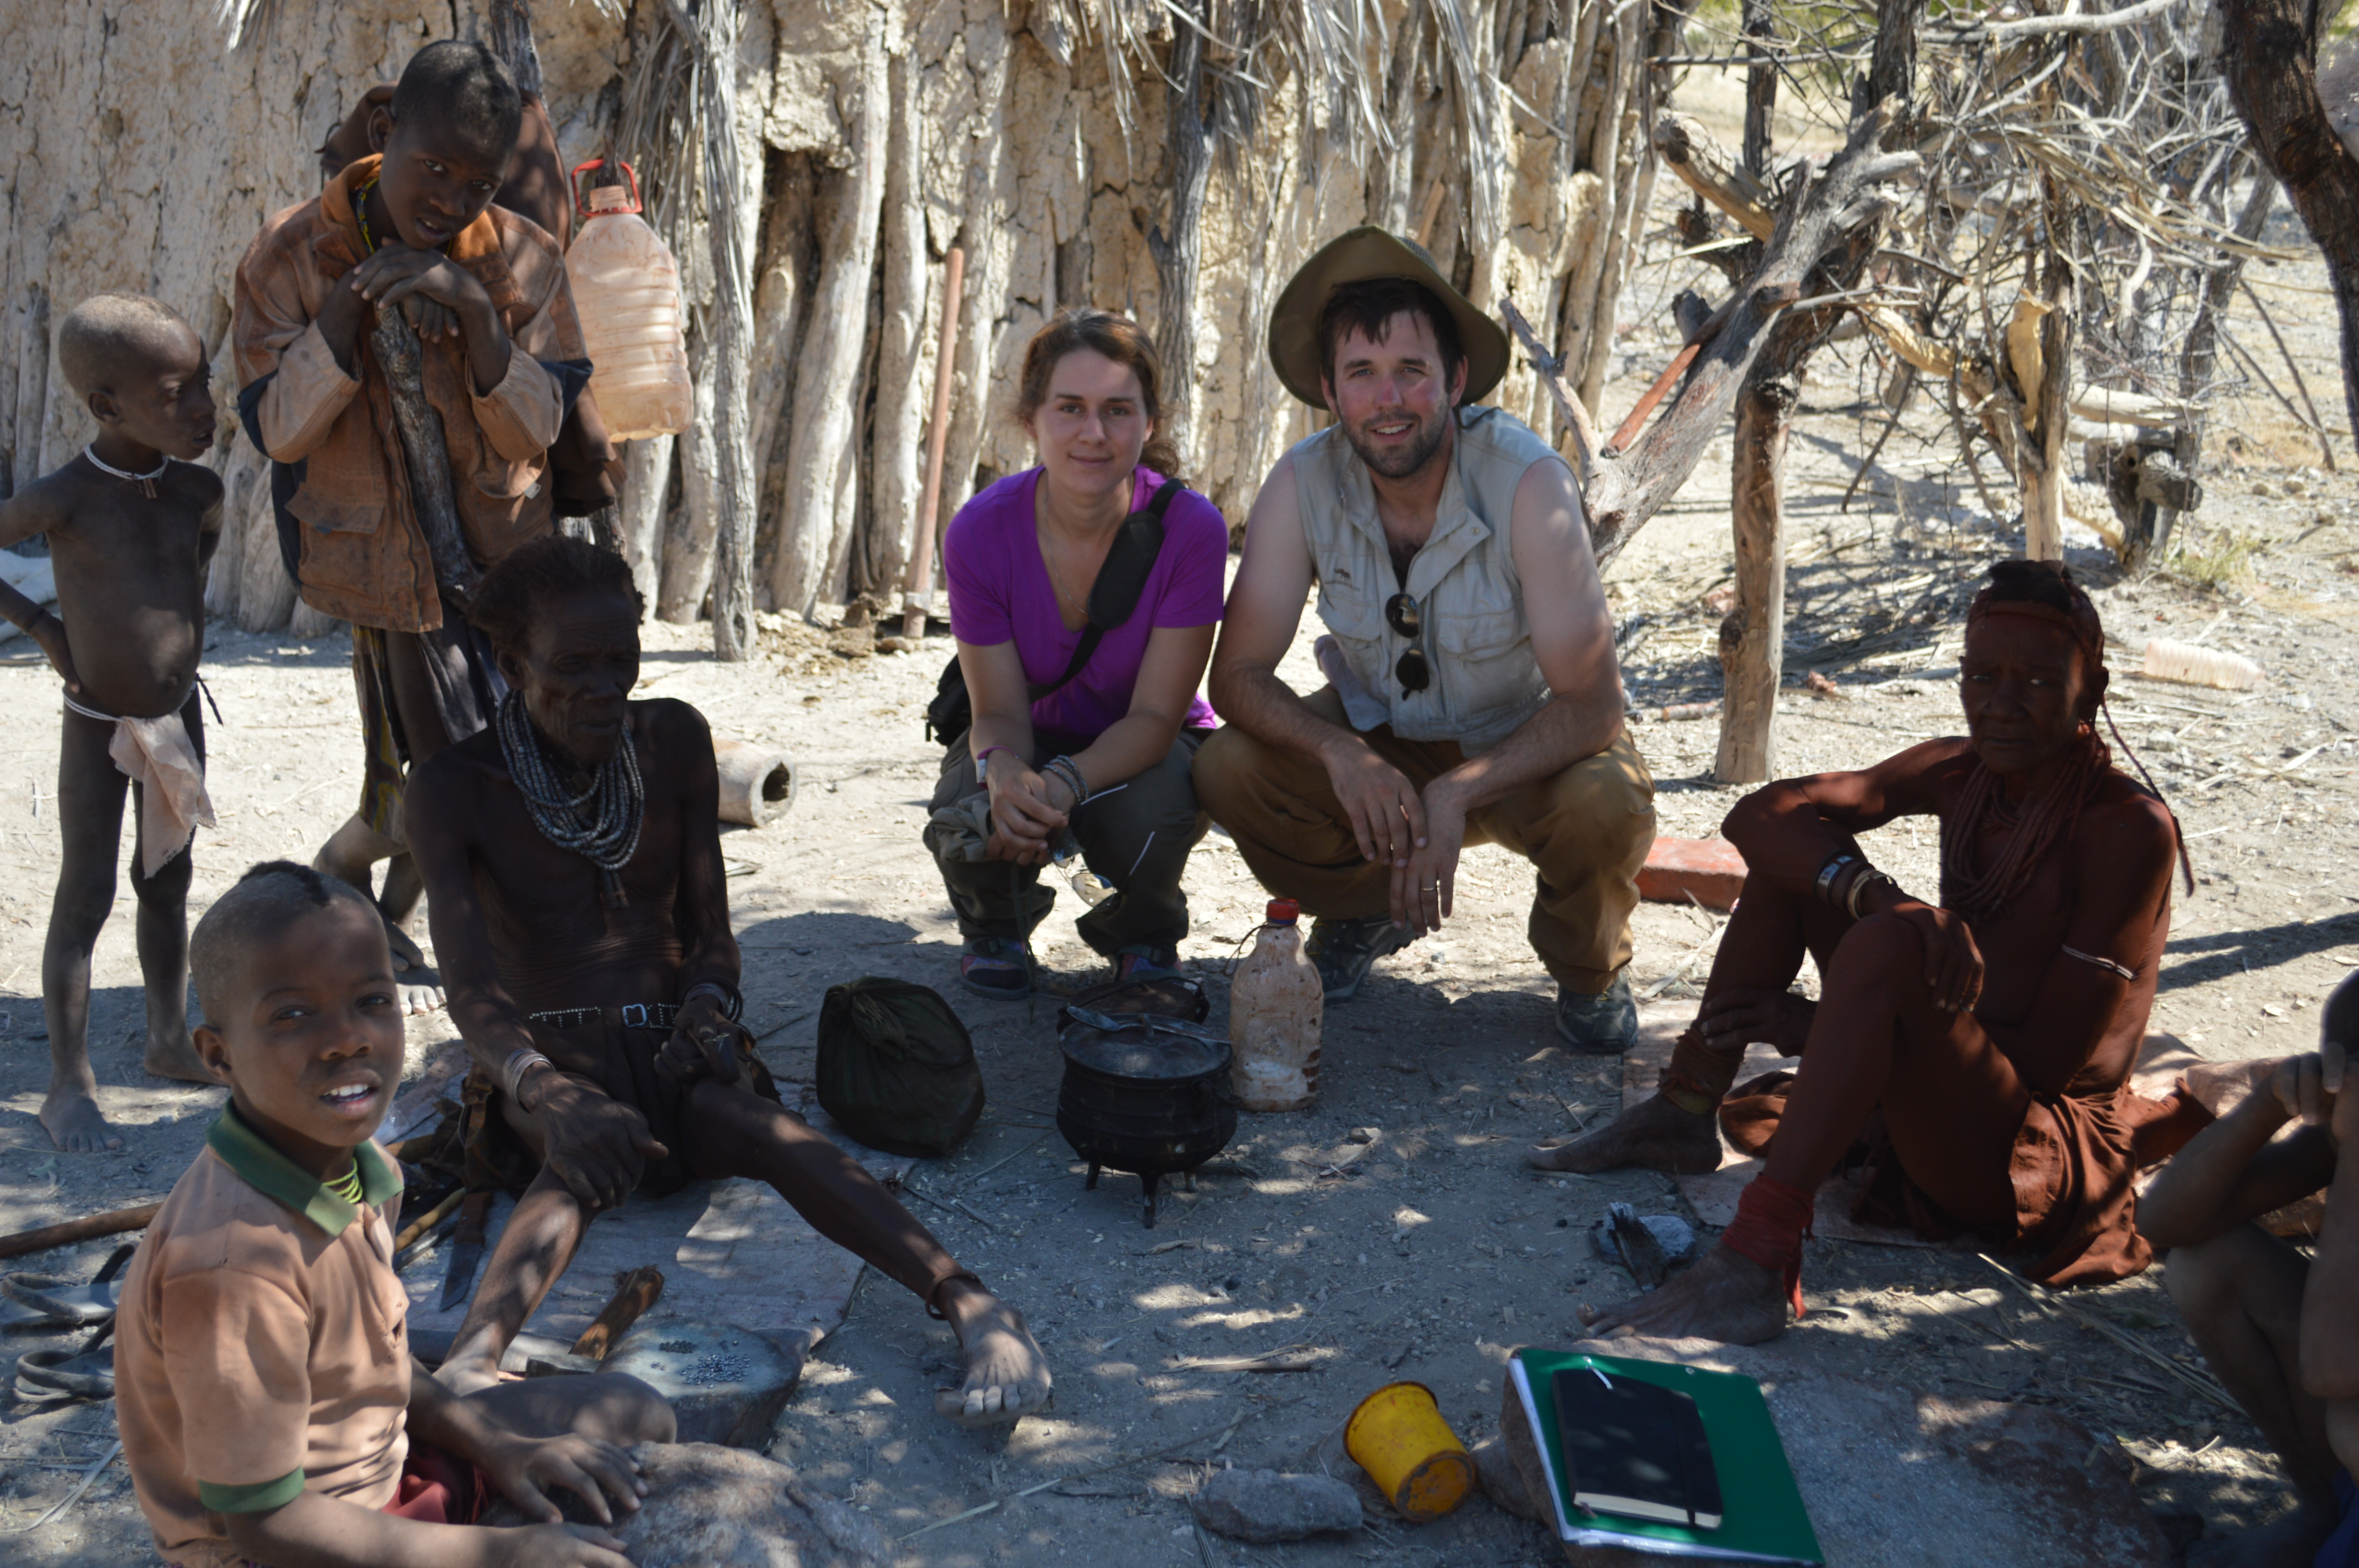
\includegraphics[width= .6\textwidth]{fieldwork}\\
\includegraphics[width= 1\textwidth]{twekids}
\end{column}

\begin{column}{.2\textwidth}
\includegraphics[width= 1\textwidth]{NSF_logo}\\
\vspace{0.75cm} 
\includegraphics[width= 1\textwidth]{SCAN_logo}
\end{column}
\end{columns}

\end{frame}

%----------------------------------------------------------------------------------------

\end{document}